\begin{center}
\tikzset{
    main node/.style={
        circle, 
        draw, 
        fill=blue!20, 
        inner sep=1pt, 
        font=\scriptsize, 
        minimum size=6mm, 
        text=black
    }
}

% Graph (a)
\begin{minipage}[t]{0.45\linewidth}
    \centering
    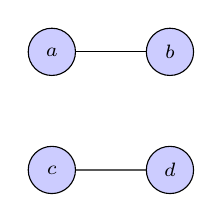
\begin{tikzpicture}[scale=1.5]
        \node[main node] (1) at (0,0) {\(a\)};
        \node[main node] (2) at (1,0) {\(b\)};
        \node[main node] (3) at (0,-1) {\(c\)};
        \node[main node] (4) at (1,-1) {\(d\)};
        \draw (1) -- (2);
        \draw (3) -- (4);
    \end{tikzpicture}
    
    \vspace{0.4em}
    {\small (a) Graphe \(G\)}
\end{minipage}%
\hfill
% Graph (b)
\begin{minipage}[t]{0.45\linewidth}
    \centering
    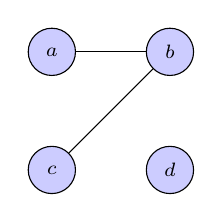
\begin{tikzpicture}[scale=1.5]
        \node[main node] (1) at (0,0) {\(a\)};
        \node[main node] (2) at (1,0) {\(b\)};
        \node[main node] (3) at (0,-1) {\(c\)};
        \node[main node] (4) at (1,-1) {\(d\)};
        \draw (1) -- (2);
        \draw (2) -- (3);
    \end{tikzpicture}
    
    \vspace{0.4em}
    {\small (b) Graphe \(H\)}
\end{minipage}

\vspace{0.8em}
\captionof{figure}{Illustration des graphes \(G\) et \(H\)}\label{fig:td1_ex1_fi1}
\end{center}